% Copyright 2026 Torbjörn E. M. Nordling
% SPDX-License-Identifier: Apache-2.0
% frame-tracking-quality.tex — Check the tracking and the rest noise (19:30–20:30)
% Figures from the supplementary: fig-wheel-overlay.pdf (15 s video of motor m1
% at duty 1.0, 3599 usable frames; frames of smallest, median, mean, largest
% angle uncertainty; (e) uncertainty against angle) and fig-rest-noise.pdf
% (\RestFrames frames at rest; share beyond omega_min = \OmegaMin rad/s is
% \RestShare %). Rest threshold rule: supplementary S6.
\begin{frame}{Check your data}{What the tracker found, and when a wheel counts as at rest}
  \scriptsize
  \begin{columns}[T]
    \column{0.4\textwidth}
    \centering
    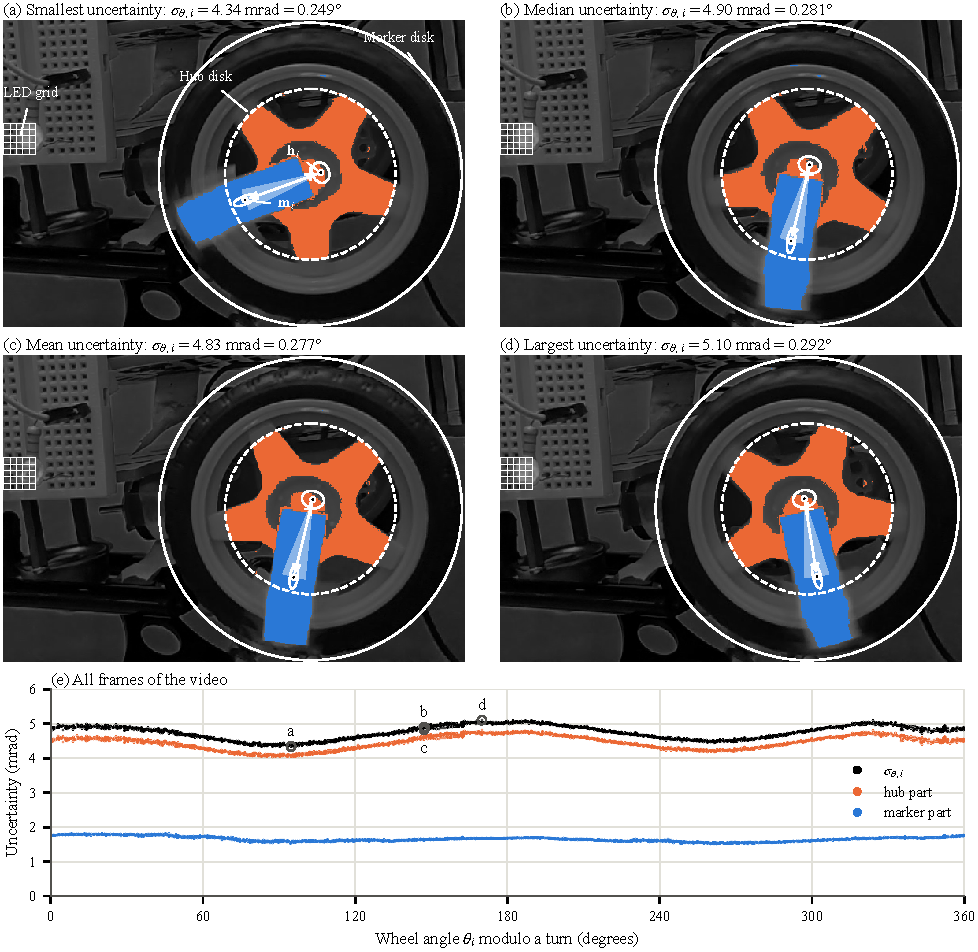
\includegraphics[width=\linewidth, height=0.66\textheight, keepaspectratio]{fig-wheel-overlay.pdf}

    Tracker output on a 15\,s video of motor m1 at duty 1.0, 3599 usable frames.
    \column{0.25\textwidth}
    \centering
    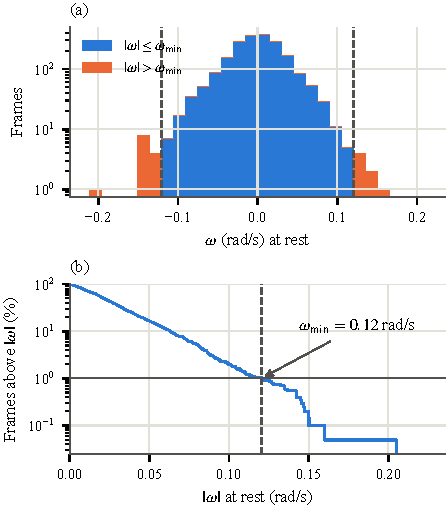
\includegraphics[width=\linewidth, height=0.66\textheight, keepaspectratio]{fig-rest-noise.pdf}

    Speed of a wheel at rest, \RestFrames{} frames.
    \column{0.31\textwidth}
    \begin{itemize}\setlength{\itemsep}{2pt}
      \item Coloured: pixels taken as marker and hub. Check that both are found, and the LED seen.
      \item A wheel at rest shows speed noise; it counts as \alert{at rest} below $\omega_{\min} = \OmegaMin$\,rad/s, exceeded by \RestShare\,\% of rest frames.
      \item Start and stop duties are judged against $\omega_{\min}$.
    \end{itemize}
  \end{columns}
\end{frame}
